\section{Zielsetzung}
Ziel dieses Versuches ist die Bestimmung der Spin-Gitter- und der Spin-Spin-Relaxationszeiten, sowie des Diffusionskoeffizienten von bidestilliertem Wasser mittels magnetischer Resonanz an Protonen.

\section{Theorie}
\subsection{Magnetisierung im thermischen Gleichgewicht}
Befindet sich eine Probe in einem statischen Magnetfeld richten sich die magnetischen Momente der Atomekerne teilweise aus, sodass eine makroskopische Magnetisierung entsteht.
Der Kernspin von Protonen beträgt $I=\textonehalf$, sodass es in einem Magnetfeld $\vec{B}=B_0\vec{e}_\text{z}$ zu einer Aufspaltung in zwei Unterniveaus mit den Quantenzahlen $m=\pm \textonehalf$ kommt.
Unter der Annahme, dass $\gamma B_0 \hbar \ll kT$ gilt, kann die Kernspinpolarisation der Protonen durch
\begin{equation}
    \langle I \rangle_\text{P} = -\frac{\hbar^2\gamma}{4kT}\,B_0
\end{equation}
genähert werden.
Die makroskopische Magnetisierung $\vec{M}$ beschreibt die Summe aller Einzelmomente pro Volumeneinheit.
Dessen Erwartungswerte in Richtung des Magnetfeldes errechnet sich im thermodynamischen Gleichgewicht bei der Temperatur $T$ zu 
\begin{equation}
    M_0=N\gamma \mu_0 \langle I \rangle_\text{P} = \frac{\mu_0\gamma^2\hbar^2N}{4kT}B_0\, .
\end{equation}
Hierbei ist $N$ die Anzahl der Momente pro Volumeneinheit und $\gamma$ das  gyromagnetisches Verhältnis von Protonen.

\subsection{Relaxationsprozesse}
Durch Einstrahlung von Hochfrequenzquanten kann die Magnetisierung aus ihrer Gleichgewichtslage $\vec{M}_0$ gebracht werden.
Der zeitliche Verlauf der darauf folgenden Relaxation wird durch die \textit{Blochschen Gleichungen} beschrieben
\begin{align}
    \frac{\mathrm{d}M_\text{x}}{\mathrm{d}t}&=\gamma B_0M_\text{y}-\frac{M_\text{x}}{T_2}\, , \label{eq:BGx} \\
    \frac{\mathrm{d}M_\text{y}}{\mathrm{d}t}&=\gamma B_0 M_\text{x} - \frac{M_\text{y}}{T_2}\, , \label{eq:BGy} \\
    \frac{\mathrm{d}M_\text{z}}{\mathrm{d}t}&=\frac{M_0-M_\text{z}}{T_1}\, . \label{eq:BGz}
\end{align}
Die beiden vorderen Terme der Gleichungen \eqref{eq:BGx} und \eqref{eq:BGy} beschreiben eine Präzessionsbewegung der Magnetisierung in der $x$-$y$-Ebene mit der Kreisfrequenz
\begin{equation}
    \omega_\text{L}=\gamma B_0\, ,
\end{equation}
welche \textit{Larmor-Frequenz} genannt wird.
Diese Präzessionbewegung bleibt auch nach der Relaxation weiterhin bestehen.
Die Relaxation der Magnetisierungskomponente in Feldrichtung wird durch die \textit{Spin-Gitter-Relaxationszeit} $T_1$ charakterisiert, während der Relaxationsprozess senkrecht zur Feldrichtung abhängig von der \textit{Spin-Spin-Relaxationszeit} $T_2$ ist.

Im Falle eines signifikant inhomogenen Feldes müssen Diffusionsprozesse durch einen zusätzlichen Term
\begin{equation}
    \frac{\partial M}{\partial t} = D \Delta M
\end{equation}
in den Blochschen Gleichungen berücksichtigt werden, wobei hier angenommen wird, dass der Gradient des Feldes konstant ist.
Die Diffusionkonstante $D$ beschreibt die thermisch bedingten Bewegungen der Spins und ist somit ein Maß für die Zeitabhängigkeit der Larmor-Frequenz, welche sich durch die Inhomogenität des Magnetfeldes ergibt.
Gemäß der Stokeschen Formel
\begin{equation}
    D=\frac{kT}{6\pi r \eta}
\end{equation}
ist die Diffusionskonstante von der Temperatur $T$, dem Molekülradius $r$ und der Viskosität $\eta$ abhängig.

\subsection{Messung der Zeitkonstanten}
Um die Magnetisierung aus ihrer Gleichgewichtslage zu bringen wird die Probe in ein Hochfrequenzfeld mit der Frequenz $\omega_\text{L}$ gebracht, dessen magnetischer Feldvektor $\vec{B}_1$ stets senkrecht zur Feldrichtung $\vec{B}$ des statisches Feldes ist.
Je länger der Puls des Hochfrequenzfeldes, desto stärker wird die Magnetisierung aus ihrer Gleichgewichtslage gedreht.
Bei einem Puls der Einstrahlungszeit 
\begin{equation}
    \Delta t_{90}=\frac{\pi}{2\gamma B_1} 
\end{equation}
wird die Magnetisierung um $90°$ gedreht.
Dementsprechend wird durch die doppelte Einstrahlungszeit $\Delta t_{180}=2 \Delta t_{90}$ eine Drehung um $180°$ erzielt.

Der Grad der Magnetisierung wird in diesem Versuch über die Induktionspannung einer Spule gemessen.
Hierzu wird die Probe zwischen die Polshuhe eines Elektromagneten gebracht und von einer Spule umschlossen, wie es in Abbildung \ref{fig:fig1} dargestellt ist.
Durch die Präzessionsbewegungen der Spins entsteht eine Induktionsspannung, welche Rückschlüsse auf die Magnetisierung der Probe erlaubt.

\begin{figure}[H]
\centering
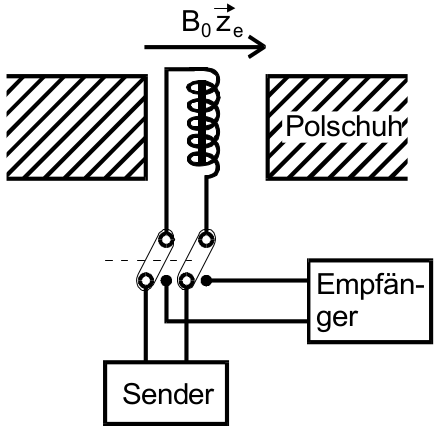
\includegraphics[width=0.4\linewidth]{figs/Aufbau}
\caption{Schematischer Versuchsaufbau. \cite{Finke}}
\label{fig:fig1}
\end{figure}

Zur Bestimmung der Spin-Gitter-Relaxationzeit $T_1$ wird die Pulsmethode verwendet.
Hierzu wird die Probe zunächst einem $180°$-Puls und nach einer Relaxationphase der Dauer $\tau$ einem $90°$-Puls ausgesetzt.
Aus den Blochschen-Gleichungen folgt, dass die zum Feld parallele Magnetisierungskomponente $M_\text{z}$ die $\tau$-Abhängigkeit
\begin{equation}
    M_\text{z}(\tau)=M_0\left(1-2\exp(-\frac{\tau}{T_1})\right)
    \label{eq:t1}
\end{equation}
aufweist.

Die Bestimmung der Spin-Spin-Relaxationszeit $T_2$ erfolgt mittels der sogenannten \textit{Meiboom-Gill-Methode}, welche eine Erweiterung der Spin-Echo-Methode darstellt.
Bei der Spin-Echo-Methode wird die Magnetisierung zunächst mit einem $90°$-Puls aus ihrer Gleichgewichtslage gebracht, sodass die einzelnen Spins um die $z$-Achse präzedieren.
Da ein reales Magnetfeld zwangsläufig leichte Inhomogenitäten aufweist, präzedieren nicht alle Spins mit derselben Larmor-Frequenz $\omega_\text{L}$, sodass die einzelnen Spins auseinanderstreben bis keine Induktionsspannung mehr gemessen werden kann.
Nach einer Zeitspanne $\tau$ werden die Spins durch einen $180°$-Puls reflippt, sodass diese nun wieder aufeinander zulaufen.
Sobald die Spins sich wieder in Phase befinden kommt es zu einem weiteren Messsignal, welches als \textit{Hahn-Echo} bezeichnet wird.

Folgen auf dem $90°$-Puls mehrere $180°$-Pulse im zeitlichen Abstand von $2\tau$, kommt es nach jedem dieser Pulse erneut zu einem Echo.
Hierbei nimmt die Amplitude des Echos exponentiell mit der Zeitkonstanten $T_2$ ab
\begin{equation}
    M_\text{y}(t)=M_0\exp(-\frac{t}{T_2}) + M_1\, . \label{eq:t2}
\end{equation}
Damit sich Abweichungen, welche durch eine Fehljustierung des $180°$-Pulses ergeben, nicht systematisch aufsummieren, werden die Schwingungen des $180°$-Pulses gegenüber des $90°$-Pulses um $90°$ in der Phase verschoben.
Somit wird erreicht, dass sich diese Abweichungen bei jedem geradzahligen Echo herauskürzen.

\subsection{Messung der Diffusionskonstante}
Weist das Magnetfeld einen signifikanten Gradienten $G$ auf, nimmt die Echo-Amplitude schneller ab, als in Gleichung \eqref{eq:t2} beschrieben und Diffusionsprozesse können nicht mehr vernachlässigt werden.
Die Amplitude der Echos wird dann durch eine weitere Zeitkonstanten
\begin{equation}
    T_\text{D}=\frac{3}{D\gamma^2 G^2\tau^2} 
\end{equation}
bestimmt, sodass diese mit der Funktion
\begin{equation}
    M_\text{y}=M_0\exp(-\frac{t}{T_2})\exp(-\frac{t}{T_\text{D}}) \stackrel{t=2\tau}{=} M_0\exp(-\frac{t}{T_2})\exp(-\frac{1}{12}D\gamma^2 G^2 t^3)
    \label{eq:echo}
\end{equation}
abnimmt.




